\documentclass[aspectratio=169,11pt]{beamer}

\usepackage[english]{babel}
\usepackage[utf8]{inputenc}
\usepackage[T1]{fontenc}
\usepackage{booktabs}
\usepackage{graphicx}
\usepackage{amsmath}
\usepackage{array}
\usepackage{xcolor}
\usepackage{hyperref}
\usepackage{tikz}

% Clean adaptation of the supplied minimal Beamer template.
\usetheme{default}
\usecolortheme{default}
\usefonttheme{professionalfonts}
\setbeamertemplate{navigation symbols}{}
\setbeamertemplate{caption}[numbered]
\setbeamertemplate{footline}{%
  \leavevmode%
  \hbox{%
    \begin{beamercolorbox}[wd=.86\paperwidth,ht=2.6ex,dp=1.1ex,leftskip=1em]{author in head/foot}%
      \insertshorttitle
    \end{beamercolorbox}%
    \begin{beamercolorbox}[wd=.14\paperwidth,ht=2.6ex,dp=1.1ex,center]{date in head/foot}%
      \insertframenumber/\inserttotalframenumber
    \end{beamercolorbox}%
  }%
}

\definecolor{hhublue}{RGB}{0,70,127}
\definecolor{hhulight}{RGB}{225,239,249}
\definecolor{goodgreen}{RGB}{38,120,82}
\definecolor{warnred}{RGB}{168,45,55}
\setbeamercolor{structure}{fg=hhublue}
\setbeamercolor{frametitle}{fg=hhublue}
\setbeamercolor{title}{fg=hhublue}
\setbeamercolor{block title}{fg=white,bg=hhublue}
\setbeamercolor{block body}{bg=hhulight!60}
\setbeamerfont{frametitle}{series=\bfseries,size=\Large}
\setbeamerfont{title}{series=\bfseries,size=\LARGE}
\setbeamersize{text margin left=0.65cm,text margin right=0.65cm}

% Plot placeholders are deliberately explicit so W&B exports can be dropped in later.
% Replace a placeholder with, for example:
% \includegraphics[width=0.92\textwidth]{figures/optimizer-trajectories.pdf}
\newcommand{\wandbplaceholder}[2]{%
  \begin{center}
    \setlength{\fboxsep}{10pt}%
    \fcolorbox{hhublue}{hhulight}{%
      \parbox[c][0.40\textheight][c]{0.88\textwidth}{%
        \centering\Large\bfseries W\&B figure placeholder\\[0.6em]
        \normalsize\mdseries #1\\[0.4em]
        \scriptsize #2
      }%
    }
  \end{center}
}

\newcommand{\diagramplaceholder}[2]{%
  \begin{center}
    \setlength{\fboxsep}{10pt}%
    \fcolorbox{hhublue}{hhulight}{%
      \parbox[c][0.43\textheight][c]{0.88\textwidth}{%
        \centering\Large\bfseries Diagram placeholder\\[0.6em]
        \normalsize\mdseries #1\\[0.45em]
        \scriptsize #2
      }%
    }
  \end{center}
}

\newcommand{\smallcite}[1]{\hfill{\tiny\color{gray}#1}}

\title[GPT-Slowrun Ablation Study]{Ablation Study of a NanoGPT Slowrun Model}
\subtitle{Optimizer, architecture, and scale transfer in the Tiny Track}
\author{Ahmed Moustafa}
\institute{}
\date{Summer Semester 2026}

\begin{document}

% -----------------------------------------------------------------------------
% Title / introduction: target < 5 minutes
% -----------------------------------------------------------------------------
{
\usebackgroundtemplate{%
  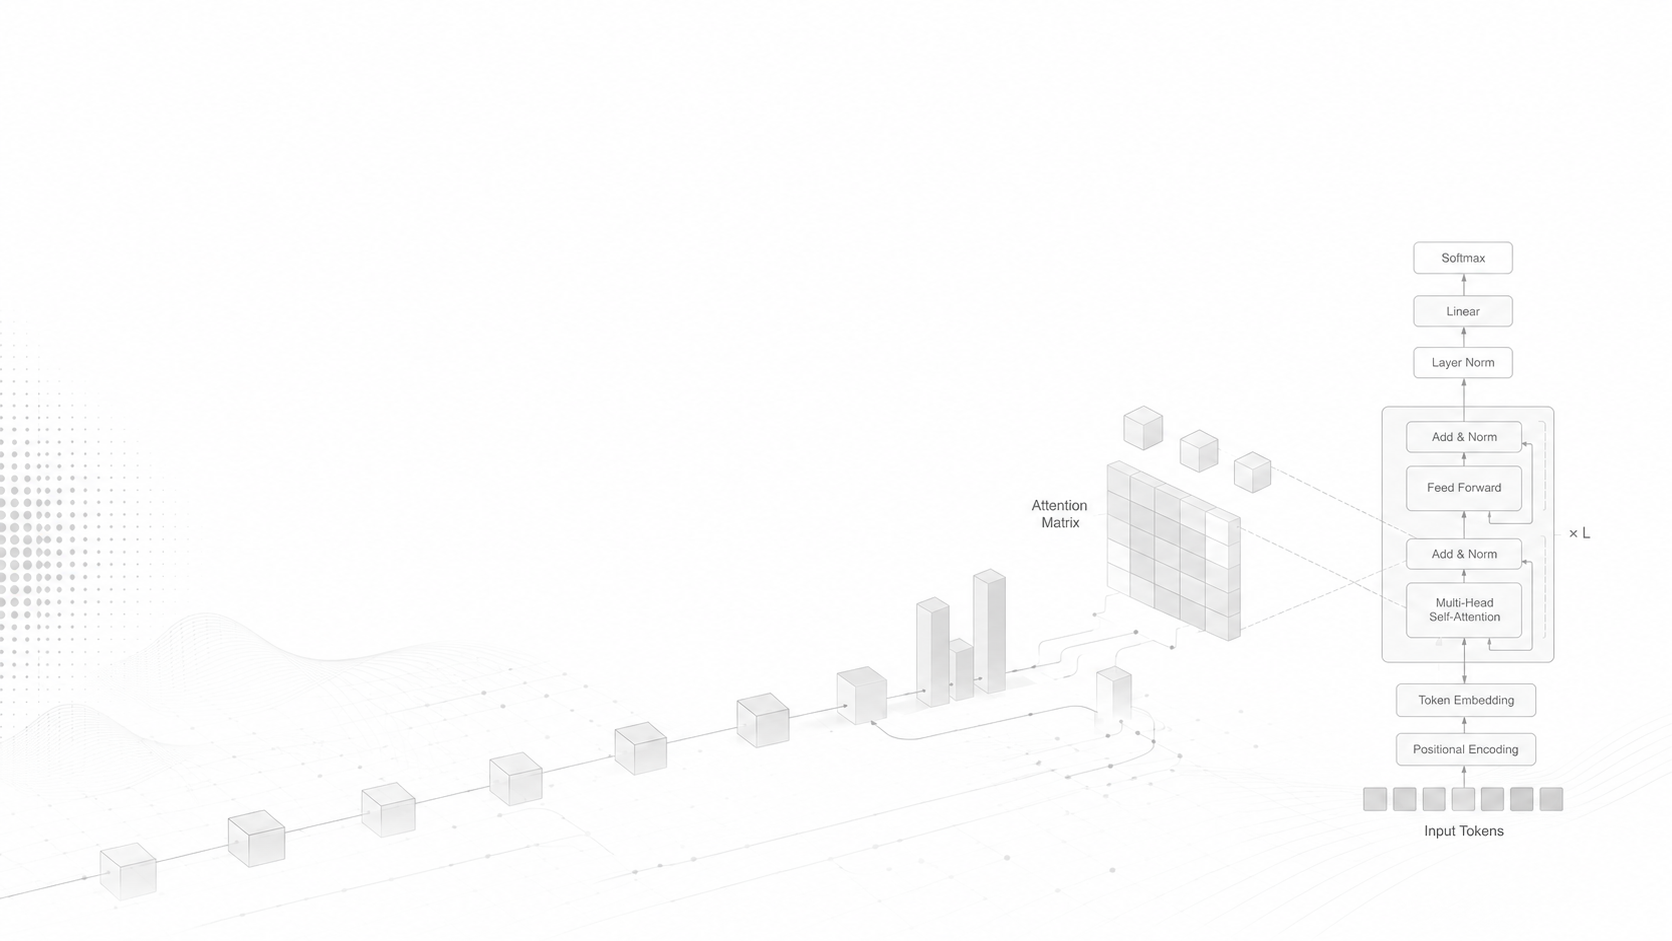
\includegraphics[width=\paperwidth,height=\paperheight]{figures/title-background.png}%
}
\begin{frame}[plain]
  \begin{tikzpicture}[remember picture,overlay]
    \node[anchor=north east,inner sep=0pt]
      at ([xshift=-0.22cm,yshift=-0.18cm]current page.north east)
      {
\includegraphics[width=0.13\paperwidth]{figures/hhu-logo.png}};
  \end{tikzpicture}
  \begin{minipage}[t][0.86\paperheight][t]{0.53\textwidth}
    \vspace{0.75cm}
    {\usebeamerfont{title}\color{hhublue}
     Ablation Study of a\\[0.12cm]NanoGPT Slowrun Model\par}
    \vspace{0.40cm}
    {\normalsize Optimizer, architecture, and scale transfer\\
     in the NanoGPT Slowrun Tiny Track\par}

    \vspace{0.52cm}
    {\color{hhublue}\rule{1.2cm}{1.1pt}}\\[0.22cm]
    {\normalsize\bfseries Ahmed Moustafa\par}
    \vspace{0.07cm}
    {\small Master Seminar: Deep Learning\enspace $\vert$\enspace SS 2026\par}
    \vspace{0.04cm}
    {\small Prof. Dr. Paul Swoboda\par}
  \end{minipage}
\end{frame}
}

\begin{frame}{Problem Statement}
  \begin{columns}[T,onlytextwidth]
    \column{0.47\textwidth}
      \begin{block}{NanoGPT Slowrun}
        \begin{itemize}
          \item 100M training tokens from FineWeb
          \item held-out validation loss is the target
          \item repeated epochs and strong regularization are allowed
        \end{itemize}
      \end{block}
    \column{0.49\textwidth}
      \begin{block}{Tiny Track used here}
        \begin{itemize}
          \item approximately 300M-parameter GPT recipe
          \item designed for a single 8$\times$H100 node
          \item Muon, modern attention components, EMA, and SWA
        \end{itemize}
      \end{block}
  \end{columns}
  \vspace{0.35cm}
  \begin{block}{How this project uses it}
    The Tiny Track code is the experimental starting point. It is reduced to
    laptop scale for screening, then selected findings are tested again on H100s.
  \end{block}
  \smallcite{Slowrun benchmark \cite{slowrun2026}; fixed-data pre-training \cite{kim2025infinite}}
\end{frame}

\begin{frame}{Research Question}
  \begin{center}
    \Large Can a 4-layer model on one laptop GPU identify choices that remain
    useful for a 16-layer model on 8 H100 GPUs?
  \end{center}
  \vspace{0.5cm}
  \begin{columns}[T]
    \column{0.48\textwidth}
      \textbf{Phase 1: inexpensive screening}
      \begin{itemize}
        \item 66M parameters, 10M train tokens
        \item optimizer and hyperparameter ablations
        \item architectural component removal
      \end{itemize}
    \column{0.48\textwidth}
      \textbf{Phase 2: scaling test}
      \begin{itemize}
        \item 317M parameters, 100M train tokens
        \item four 8$\times$H100 runs
        \item test whether the apparent winners transfer
      \end{itemize}
  \end{columns}
  \vspace{0.3cm}
  \alert{Preview: the strongest small-scale result reverses after scaling.}
\end{frame}

\begin{frame}{GPT Overview}
  \begin{center}
    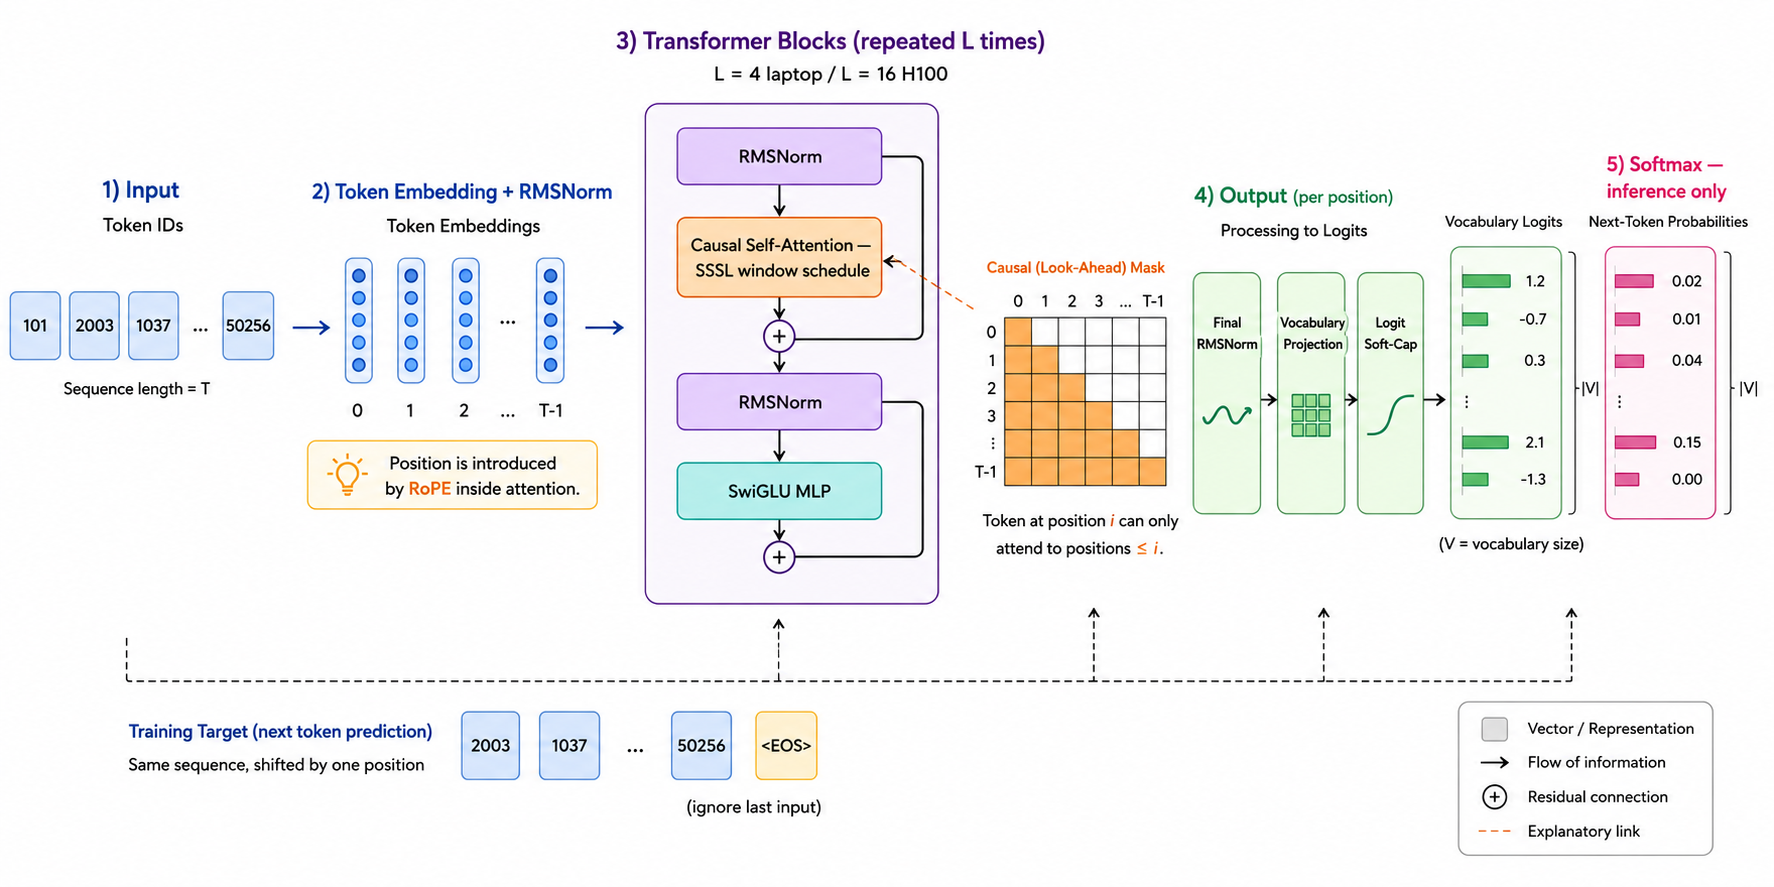
\includegraphics[width=0.99\textwidth,height=0.79\textheight,keepaspectratio]
      {figures/gpt-simple.png}
  \end{center}
  \vspace{-0.25cm}
  \smallcite{Decoder-only Transformer foundation \cite{vaswani2017attention}}
\end{frame}

% -----------------------------------------------------------------------------
% Method / technical insight: target > 50% of speaking time
% -----------------------------------------------------------------------------
\begin{frame}{Leaderboard Architecture}
  \small
  \begin{tabular}{>{\bfseries}p{0.22\textwidth}p{0.70\textwidth}}
    \toprule
    Component & Recipe used in this study \\
    \midrule
    Backbone & Decoder-only Transformer with causal self-attention \cite{vaswani2017attention} \\
    Position & Half-truncated rotary embeddings; partial key offset \cite{su2021roformer} \\
    Information paths & Residual stream, U-Net skips, gated value residuals \cite{zhou2024resformer} \\
    Head control & Learnable per-head attention gate \\
    Optimizer & Muon for matrix parameters; AdamW for embeddings and scalars \\
    Late training & EMA plus four-epoch checkpoint averaging / SWA \cite{izmailov2018swa} \\
    Data & GPT-2 tokenizer; FineWeb training and held-out validation tokens \\
    \bottomrule
  \end{tabular}
  \vspace{0.4cm}
  \begin{center}
    Our contribution is a controlled ablation and scale-transfer study of this recipe.
  \end{center}
\end{frame}

\begin{frame}{Baseline Architecture}
  {\centering
    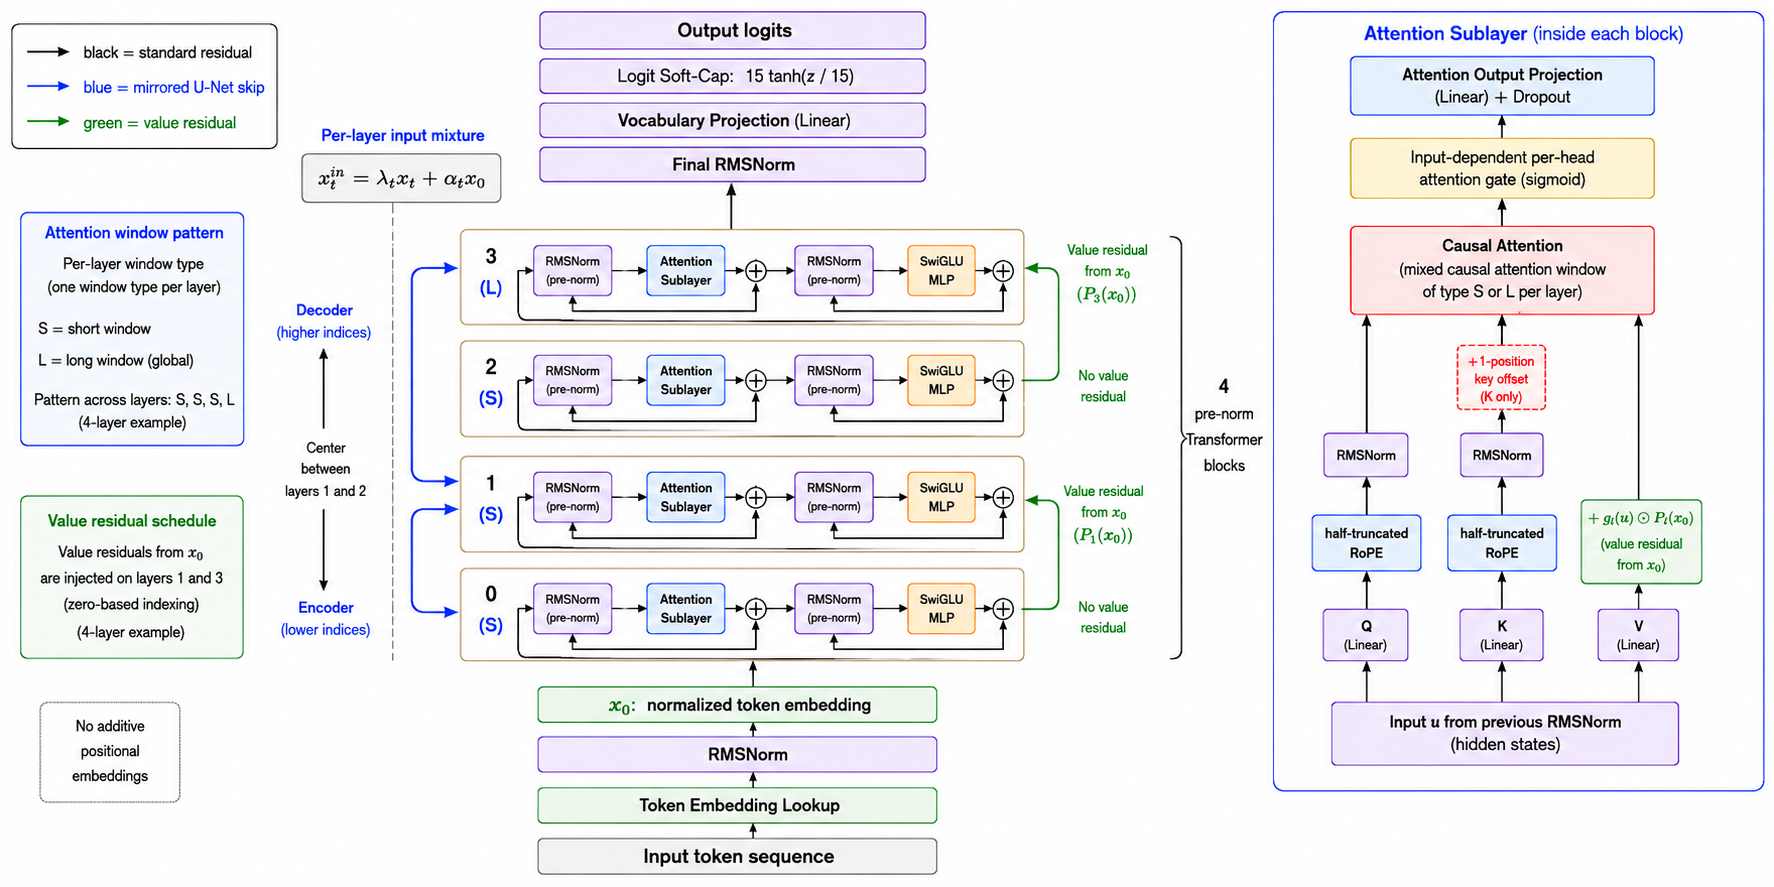
\includegraphics[width=0.965\textwidth,height=0.765\textheight,keepaspectratio]
      {figures/gpt-detailed.png}
    \par}
\end{frame}

\begin{frame}{Architecture Components}
  \begin{columns}[T]
    \column{0.48\textwidth}
      \textbf{Attention path}
      \begin{itemize}
        \item half-truncated RoPE
        \item partial key offset
        \item per-head output gate
        \item causal local/global attention pattern
      \end{itemize}
    \column{0.48\textwidth}
      \textbf{Cross-layer paths}
      \begin{itemize}
        \item standard residual connection
        \item learnable U-Net skip weights
        \item projected input $x_0$ injected into values
        \item alternating value-residual layers
      \end{itemize}
  \end{columns}
  \vspace{0.5cm}
  \begin{block}{Ablation principle}
    Remove or alter one component while holding the data, optimizer, schedule,
    and evaluation pipeline fixed.
  \end{block}
\end{frame}

\begin{frame}{Value Residuals}
  \begin{columns}[c]
    \column{0.54\textwidth}
      Standard value projection:
      \[
        V_\ell = X_\ell W^V_\ell
      \]
      Value-residual variant used here:
      \[
        \widetilde{V}_\ell = V_\ell + g_\ell(X_\ell)\odot P_\ell(X_0)
      \]
      The initial token representation remains directly accessible to later
      attention layers.
    \column{0.42\textwidth}
      \begin{block}{Why ablate it?}
        It adds both a new information path and about 0.8\% more parameters at
        small scale. A loss change cannot be attributed to connectivity alone.
      \end{block}
  \end{columns}
  \smallcite{Value residual learning / ResFormer \cite{zhou2024resformer}}
\end{frame}

\begin{frame}{Muon Optimizer}
  \begin{columns}[T]
    \column{0.49\textwidth}
      \textbf{Momentum}
      \[
        M_t = \beta M_{t-1} + G_t
      \]
      \textbf{Orthogonalized direction}
      \[
        O_t \approx M_t(M_t^\top M_t)^{-1/2}
      \]
      Five Newton--Schulz-style iterations approximate the polar factor.
    \column{0.47\textwidth}
      \textbf{Parameter update}
      \[
        W_{t+1}=(1-\eta_t\lambda_t)W_t-\eta_t O_t
      \]
      \begin{itemize}
        \item matrix structure is preserved
        \item singular directions are rescaled
        \item computation is more expensive than AdamW
      \end{itemize}
  \end{columns}
  \smallcite{Muon implementation and algorithm \cite{jordan2024muon}}
\end{frame}

\begin{frame}{Hybrid Optimizer}
  \small
  \begin{tabular}{p{0.31\textwidth}p{0.20\textwidth}p{0.19\textwidth}p{0.20\textwidth}}
    \toprule
    Parameter group & Optimizer & Base LR & LR at multiplier 0.8 \\
    \midrule
    Hidden matrices & Muon & 0.040 & 0.032 \\
    Embeddings & AdamW & 0.150 & 0.120 \\
    Scalar / gate parameters & AdamW & 0.250 & 0.200 \\
    Unembedding head & AdamW & 0.001 & 0.0008 \\
    \bottomrule
  \end{tabular}
  \vspace{0.6cm}
  \begin{block}{Fair optimizer comparison}
    The AdamW-only variant keeps the architecture, data order, schedules,
    evaluation, EMA, and SWA unchanged; only matrix-parameter optimization changes.
  \end{block}
  \smallcite{AdamW \cite{loshchilov2019adamw}; Muon parameter grouping \cite{jordan2024muon}}
\end{frame}

\begin{frame}{Training Schedule}
  \begin{columns}[T]
    \column{0.52\textwidth}
      \textbf{Weight decay schedule}
      \begin{enumerate}
        \item hold the configured value through epoch 2
        \item decay toward 0.1 through epoch 8
        \item ramp toward 1.25 by epoch 16
      \end{enumerate}
      \textbf{Last four epochs}
      \begin{itemize}
        \item cosine LR cycles create diverse checkpoints
        \item recency-weighted checkpoint average
      \end{itemize}
    \column{0.44\textwidth}
      \textbf{EMA weights}
      \[
        \bar\theta_t = \beta\bar\theta_{t-1}+(1-\beta)\theta_t
      \]
      \textbf{Checkpoint average}
      \[
        \theta_{\mathrm{avg}}=\sum_{j=1}^{4}
        \frac{j}{1+2+3+4}\theta_j
      \]
  \end{columns}
  \vspace{0.3cm}
  These mechanisms interact; weight decay cannot be interpreted independently
  of the late-training schedule.
\end{frame}

\begin{frame}{Checkpoint Averaging}
  \small
  Token-level cross-entropy masks padding and uses the same held-out data for
  every run:
  \[
    \mathcal{L}_{\mathrm{val}}=
    \frac{\sum_i \mathrm{CE}_i\,\mathbb{1}[t_i\neq\mathrm{PAD}]}
         {\sum_i \mathbb{1}[t_i\neq\mathrm{PAD}]}
  \]
  \begin{columns}[T]
    \column{0.32\textwidth}
      \textbf{Raw}\par
      End of every epoch
    \column{0.32\textwidth}
      \textbf{EMA}\par
      Evaluated after training
    \column{0.32\textwidth}
      \textbf{Checkpoint average}\par
      Last four epochs
  \end{columns}
  \vspace{0.5cm}
  \begin{block}{Reported ``best'' loss}
    Minimum over raw epoch checkpoints, EMA, and checkpoint average. The winning
    checkpoint type is always reported alongside the value.
  \end{block}
\end{frame}

\begin{frame}{Evaluation Metric}
  \begin{columns}[c]
    \column{0.47\textwidth}
      \textbf{Per-token negative log-likelihood}
      \[
        \ell_i=-\log p_\theta(t_i\mid t_{<i})
      \]
      \textbf{Masked validation loss}
      \[
        \mathcal{L}_{\mathrm{val}}=
        \frac{\sum_i \ell_i\,m_i}{\sum_i m_i},
        \qquad m_i=\mathbb{1}[t_i\neq\mathrm{PAD}]
      \]
    \column{0.49\textwidth}
      \setlength{\fboxsep}{8pt}%
      \fcolorbox{hhublue}{hhulight}{%
        \parbox[c][0.34\textheight][c]{0.88\linewidth}{%
          \centering\large\bfseries Metric diagram placeholder\\[0.5em]
          \scriptsize Show input tokens and shifted targets, one highlighted
          next-token probability, padding masked out, and three model-weight
          sources feeding the same evaluator: raw, EMA, and checkpoint average.
        }%
      }
  \end{columns}
  \vspace{0.35cm}
  Lower loss means the model assigns more probability to the observed validation tokens.
\end{frame}

\begin{frame}{Ablation Study Outline}
  \small
  \begin{columns}[T]
    \column{0.47\textwidth}
      \textbf{Training recipe ablations}
      \begin{itemize}
        \item LR multiplier: 0.4, 0.8, 1.0
        \item weight decay: 0.2, 0.8, 1.2
        \item dropout: 0.0, 0.1, 0.2
        \item document shuffle: on / off
        \item Muon+AdamW versus AdamW-only
      \end{itemize}
    \column{0.49\textwidth}
      \textbf{Architecture ablations}
      \begin{itemize}
        \item remove or modify attention gate
        \item remove U-Net skips
        \item remove value residuals
        \item remove partial key offset
        \item full RoPE plus no key offset
      \end{itemize}
  \end{columns}
  \vspace{0.4cm}
  \alert{Limitation: one run per configuration means small differences are descriptive, not statistically resolved.}
\end{frame}

\begin{frame}{Experiment Scaling}
  \small
  \begin{tabular}{p{0.31\textwidth}cc}
    \toprule
    & Laptop screening & H100 scaling test \\
    \midrule
    Transformer & 4 layers, 512 dim & 16 layers, 1024 dim \\
    Parameters & 65.7M & 316.9M \\
    Train / validation tokens & 10M / 1M & 100M / 10M \\
    Sequence length & 2048 & 2048 \\
    Effective batch tokens & 16,384 & 524,288 \\
    Hardware & 1$\times$ RTX 3050 4GB & 8$\times$ H100 \\
    Epochs & 16 & 16 \\
    \bottomrule
  \end{tabular}
  \vspace{0.5cm}
  Same optimizer family, architecture family, evaluation code, and late-training
  averaging; model size, data, batch size, and hardware change together.
\end{frame}

\begin{frame}{Effective Batch Size}
  \begin{center}
    \Large
    $16$ sequences/GPU $\times$ $2048$ tokens $\times$ $8$ GPUs\\[0.3em]
    $=262{,}144$ tokens per micro-step
  \end{center}
  \vspace{0.4cm}
  \begin{center}
    Two accumulated micro-steps\\[0.3em]
    $\Rightarrow 524{,}288$ tokens per optimizer update
  \end{center}
  \vspace{0.5cm}
  \begin{block}{Why this matters}
    Batch size and model width change the optimization regime. A hyperparameter
    that wins on the laptop is a hypothesis for scaling, not a guaranteed winner.
  \end{block}
\end{frame}

% -----------------------------------------------------------------------------
% Experiments: target 20--30% of speaking time
% -----------------------------------------------------------------------------
\begin{frame}{Phase 1: Optimizer Ablation}
  \small
  \begin{tabular}{p{0.31\textwidth}ccc}
    \toprule
    Optimizer & LR multiplier & Best val loss & Outcome \\
    \midrule
    \textbf{Muon + AdamW} & 0.8 & \textbf{4.7624} & stable \\
    AdamW only & 0.8 & 6.1809 & diverged at step 1,626 \\
    AdamW only & 0.6 & 4.8975 & stable \\
    \bottomrule
  \end{tabular}
  \vspace{0.6cm}
  \begin{columns}[T]
    \column{0.48\textwidth}
      \textbf{Observed}
      \begin{itemize}
        \item high-LR AdamW produced NaNs
        \item lowering LR restored stability
        \item stable AdamW remained 0.135 loss worse
      \end{itemize}
    \column{0.48\textwidth}
      \textbf{Careful interpretation}
      \begin{itemize}
        \item consistent with Muon's bounded update geometry
        \item gradient/update norms were not logged
        \item exact failure mechanism remains a hypothesis
      \end{itemize}
  \end{columns}
\end{frame}

\begin{frame}{Optimizer Training Curves}
  \begin{columns}[T,onlytextwidth]
    \column{0.495\textwidth}
      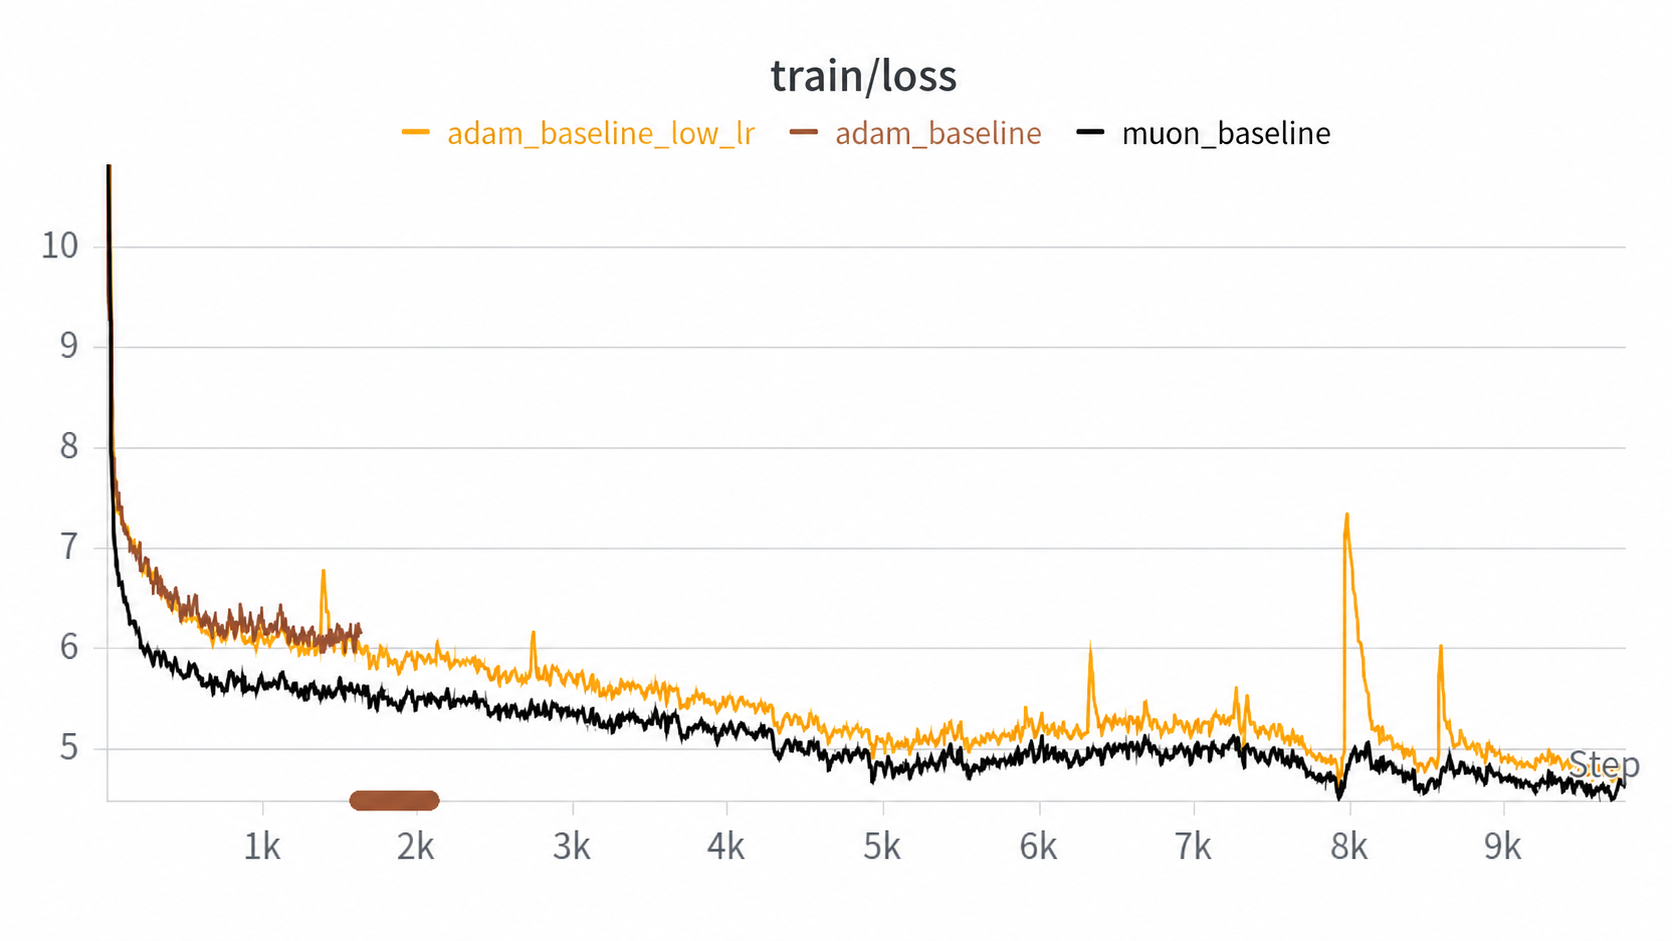
\includegraphics[width=\linewidth]{figures/graphs/moun_vs_adam_train_loss.png}
    \column{0.495\textwidth}
      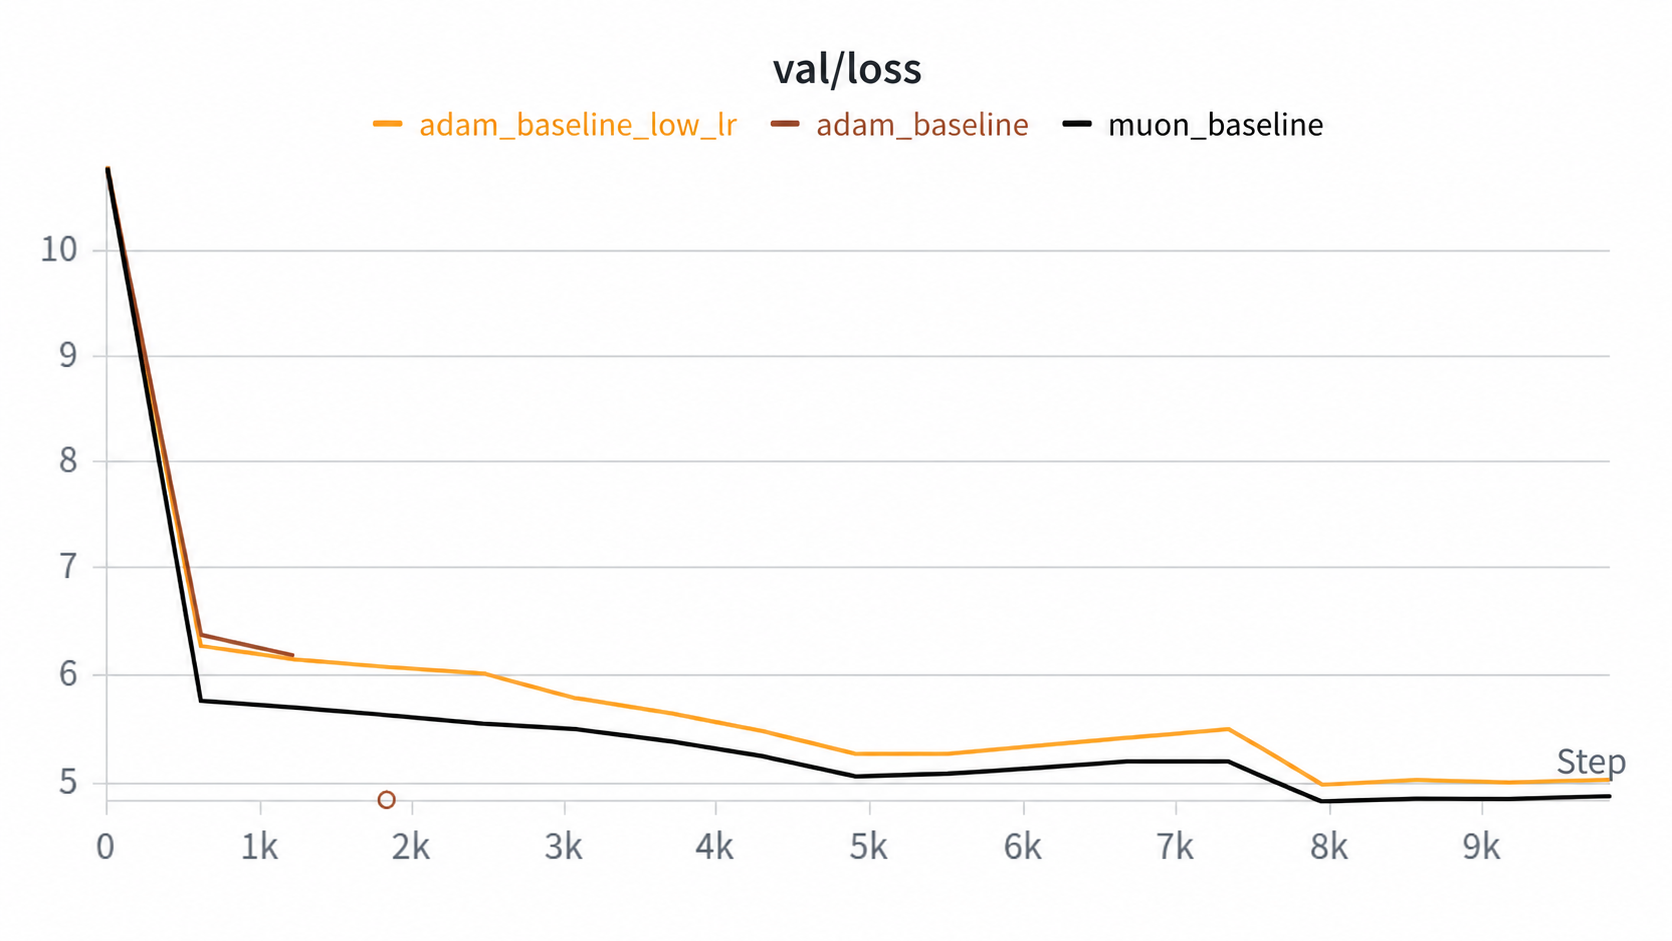
\includegraphics[width=\linewidth]{figures/graphs/moun_vs_adam_val_loss.png}
  \end{columns}
  \vspace{0.25cm}
  \begin{center}
    \small AdamW at LR multiplier 0.8 stops at step 1,626 after producing NaNs;
    Muon remains stable through training.
  \end{center}
\end{frame}

\begin{frame}{Phase 2: Hyperparameter Ablation}
  \small
  \begin{tabular}{p{0.34\textwidth}cc}
    \toprule
    Configuration & Best val loss & Change vs. baseline \\
    \midrule
    \textbf{Low WD (0.2)} & \textbf{4.4606} & \textbf{$-0.3018$} \\
    Low LR (0.4) & 4.6436 & $-0.1188$ \\
    No dropout & 4.7150 & $-0.0474$ \\
    No shuffle & 4.7597 & $-0.0027$ \\
    Baseline & 4.7624 & -- \\
    High dropout & 4.7854 & $+0.0230$ \\
    High LR (1.0) & 4.8138 & $+0.0514$ \\
    High WD (1.2) & 4.9253 & $+0.1629$ \\
    \bottomrule
  \end{tabular}
  \vspace{0.3cm}
  Low WD improves best loss by 6.3\% on the 66M-parameter screen.
\end{frame}

\begin{frame}{Hyperparameter Training Curves}
  \wandbplaceholder
    {Validation loss by epoch for baseline, LR-low, and WD-low}
    {Runs: baseline 3pzf3l2k; LR-low 79wkc6pa; WD-low yfhvegka. Use three colors only; distinguish raw epoch loss from final EMA/SWA markers.}
\end{frame}

\begin{frame}{Phase 3: Architecture Ablation}
  \small
  \begin{tabular}{p{0.38\textwidth}cc}
    \toprule
    Variant & Best val loss & Change vs. baseline \\
    \midrule
    No attention gate & 4.7555 & $-0.0069$ \\
    Baseline & 4.7624 & -- \\
    No U-Net skips & 4.7642 & $+0.0018$ \\
    Full RoPE + no key offset & 4.7708 & $+0.0084$ \\
    No key offset & 4.7778 & $+0.0154$ \\
    Strong gate & 4.7802 & $+0.0178$ \\
    \textbf{No value residual} & \textbf{4.8079} & \textbf{$+0.0456$} \\
    \bottomrule
  \end{tabular}
  \vspace{0.35cm}
  Value residual removal gives the largest degradation, but it also removes
  524,800 parameters. The RoPE comparison changes two components simultaneously.
\end{frame}

\begin{frame}{Scaled Results}
  \small
  \begin{tabular}{p{0.35\textwidth}ccc}
    \toprule
    H100 configuration & WD & LR mult. & Best val loss \\
    \midrule
    \textbf{Baseline sigmoid gate} & \textbf{0.8} & \textbf{0.8} & \textbf{3.3343} \\
    Strong gate & 0.8 & 0.8 & 3.3376 \\
    Strong gate + low WD & 0.2 & 0.8 & 3.4735 \\
    Sigmoid gate + low WD & 0.2 & \alert{0.6} & 3.4836 \\
    \bottomrule
  \end{tabular}
  \vspace{0.5cm}
  \begin{itemize}
    \item The controlled strong-gate pair shows a $+0.1360$ loss penalty from low WD.
    \item Gate choice is negligible at WD 0.8: only $0.0033$ difference.
    \item The sigmoid low-WD run also changes LR, so it is supporting evidence only.
  \end{itemize}
\end{frame}

\begin{frame}{Scaling Curves}
  \wandbplaceholder
    {H100 validation loss or BPB by epoch, with epoch 13 highlighted}
    {Overlay: baseline vryw9bxv; strong gate vp6dxkif; strong+low-WD 1l93yfpf; sigmoid+low-WD cy7besr1. Shade epochs 13--16 as the SWA/cosine-cycle phase.}
\end{frame}

\begin{frame}{Weight Decay and SWA}
  \begin{columns}[T]
    \column{0.48\textwidth}
      \textbf{WD 0.8 runs}
      \begin{itemize}
        \item raw loss continues to improve late
        \item checkpoint averaging gives the best result
        \item final best loss near 3.33
      \end{itemize}
    \column{0.48\textwidth}
      \textbf{WD 0.2 runs}
      \begin{itemize}
        \item best raw checkpoint occurs at epoch 8
        \item validation loss worsens in epochs 13--16
        \item EMA and averaging inherit worse late weights
      \end{itemize}
  \end{columns}
  \vspace{0.5cm}
  \begin{block}{Supported conclusion}
    Low initial WD is incompatible with this scaled recipe and late-training
    schedule. A WD-only $\times$ SWA on/off factorial experiment is still needed
    to isolate the mechanism.
  \end{block}
\end{frame}

\begin{frame}{Training Experience}
  \begin{itemize}
    \item AdamW at matrix LR 0.032 diverged; LR 0.024 completed training.
    \item Muon added Newton--Schulz compute but achieved the best small-scale loss.
    \item Laptop runs required gradient accumulation and disabled \texttt{torch.compile}.
    \item Peak laptop VRAM stayed near 4.7GB; a 16-layer model required H100 scaling.
    \item Raw, EMA, and averaged checkpoints can rank configurations differently.
    \item W\&B logs, terminal logs, JSON summaries, checkpoints, and run scripts are retained.
  \end{itemize}
  \vspace{0.4cm}
  Reproduction quality is part of the result: each table entry can be traced to
  a stored artifact or W\&B run.
\end{frame}

\begin{frame}{Limitations}
  \small
  \begin{tabular}{p{0.31\textwidth}p{0.61\textwidth}}
    \toprule
    Threat & Consequence \\
    \midrule
    One seed per setting & no empirical variance; sub-percent gaps may be noise \\
    Scale changes together & model, data, batch, hardware, and kernels are not isolated \\
    Full RoPE confound & key offset is disabled at the same time \\
    Value-residual ablation & removes both a path and 0.8\% of parameters \\
    One low-WD run uses LR 0.6 & not a controlled WD-only baseline comparison \\
    Best-of-many checkpoint metric & optimistic selection across raw/EMA/average \\
    \bottomrule
  \end{tabular}
  \vspace{0.4cm}
  These limitations narrow the claims; they do not erase the controlled
  strong-gate weight-decay reversal or the optimizer stability observation.
\end{frame}

\begin{frame}{Take-Home Message}
  \begin{enumerate}
    \item \textbf{Muon was the strongest optimizer tested.} It tolerated the
      aggressive matrix LR and beat stable AdamW at small scale.
    \item \textbf{Most architectural tweaks were minor.} Value residuals produced
      the largest observed architecture signal, with a parameter-count confound.
    \item \textbf{Small-scale tuning did not reliably transfer.} WD 0.2 improved
      laptop-scale loss by 6.3\% but degraded a controlled H100 pair by about 4\%.
    \item \textbf{Schedules must be studied as systems.} Weight decay, LR cycling,
      EMA, and checkpoint averaging interact late in training.
  \end{enumerate}
  \vspace{0.5cm}
  \begin{center}
    \Large Cheap ablations generate hypotheses; scaling experiments decide which survive.
  \end{center}
\end{frame}

\begin{frame}[allowframebreaks]{References}
  \scriptsize
  \bibliography{references}
  \bibliographystyle{apalike}
\end{frame}

\end{document}
